% Part 4: Planning -> Building Workflow
% Teaching Agentic Coding Tools to Students
% University of South Carolina Beamer Presentation

\documentclass[aspectratio=169,10pt]{beamer}

% Theme setup - Madrid with custom modifications
\usetheme{Madrid}
\useinnertheme{rectangles}
\useoutertheme{default}

% Remove rounded corners everywhere
\setbeamertemplate{blocks}[default]
\setbeamertemplate{title page}[default][colsep=-4bp,rounded=false]
\setbeamertemplate{frametitle}[default][colsep=-4bp,rounded=false]
\setbeamertemplate{navigation symbols}{}

% UofSC Color Palette
\definecolor{UofSCGarnet}{HTML}{73000A}
\definecolor{UofSCBlack}{HTML}{000000}
\definecolor{UofSCWhite}{HTML}{FFFFFF}
\definecolor{UofSCAtlantic}{HTML}{466A9F}
\definecolor{UofSCCongaree}{HTML}{1F414D}
\definecolor{UofSCHorseshoe}{HTML}{65780B}
\definecolor{UofSCRose}{HTML}{CC2E40}
\definecolor{UofSCDarkGarnet}{HTML}{570008}
\definecolor{UofSC90Black}{HTML}{363636}
\definecolor{UofSC70Black}{HTML}{5C5C5C}
\definecolor{UofSC50Black}{HTML}{A2A2A2}

% Apply UofSC colors to Beamer theme
\setbeamercolor{palette primary}{bg=UofSCGarnet,fg=UofSCWhite}
\setbeamercolor{palette secondary}{bg=UofSCCongaree,fg=UofSCWhite}
\setbeamercolor{palette tertiary}{bg=UofSCAtlantic,fg=UofSCWhite}
\setbeamercolor{palette quaternary}{bg=UofSCBlack,fg=UofSCWhite}
\setbeamercolor{structure}{fg=UofSCGarnet}
\setbeamercolor{section in toc}{fg=UofSCGarnet}
\setbeamercolor{subsection in toc}{fg=UofSCCongaree}
\setbeamercolor{title}{fg=UofSCWhite,bg=UofSCGarnet}
\setbeamercolor{frametitle}{fg=UofSCWhite,bg=UofSCGarnet}
\setbeamercolor{block title}{bg=UofSCGarnet,fg=UofSCWhite}
\setbeamercolor{block body}{bg=UofSCWhite,fg=UofSCBlack}
\setbeamercolor{block title alerted}{bg=UofSCRose,fg=UofSCWhite}
\setbeamercolor{block body alerted}{bg=UofSCWhite,fg=UofSCBlack}
\setbeamercolor{block title example}{bg=UofSCAtlantic,fg=UofSCWhite}
\setbeamercolor{block body example}{bg=UofSCWhite,fg=UofSCBlack}
\setbeamercolor{item}{fg=UofSCGarnet}
\setbeamercolor{subitem}{fg=UofSCCongaree}
\setbeamercolor{itemize item}{fg=UofSCGarnet}
\setbeamercolor{itemize subitem}{fg=UofSCCongaree}
\setbeamercolor{enumerate item}{fg=UofSCGarnet}
\setbeamercolor{enumerate subitem}{fg=UofSCCongaree}
\setbeamercolor{footnote}{fg=UofSC70Black}
\setbeamercolor{caption name}{fg=UofSCGarnet}

% Sharp corners for all boxes
\setbeamertemplate{blocks}[default]

% Packages
\usepackage{tikz}
\usetikzlibrary{shapes.geometric, arrows.meta, positioning, calc, fit, backgrounds}
\usepackage{listings}
\usepackage{booktabs}
\usepackage{array}
\usepackage{multirow}
\usepackage{graphicx}
\usepackage{xcolor}

% TikZ styles for diagrams - sharp corners only
\tikzset{
    box/.style={
        draw=UofSCBlack,
        fill=#1,
        minimum width=2.5cm,
        minimum height=0.8cm,
        text=UofSCWhite,
        font=\small\bfseries,
        align=center,
        inner sep=4pt
    },
    box/.default=UofSCGarnet,
    lightbox/.style={
        draw=UofSCBlack,
        fill=UofSCWhite,
        minimum width=2.5cm,
        minimum height=0.8cm,
        text=UofSCBlack,
        font=\small,
        align=center,
        inner sep=4pt
    },
    arrow/.style={
        ->,
        >=Stealth,
        thick,
        UofSCBlack
    },
    bigarrow/.style={
        ->,
        >=Stealth,
        line width=1.5pt,
        UofSCGarnet
    },
    phase/.style={
        draw=UofSCBlack,
        fill=#1,
        minimum width=3cm,
        minimum height=1cm,
        text=UofSCWhite,
        font=\bfseries,
        align=center
    },
    phase/.default=UofSCGarnet,
    subphase/.style={
        draw=UofSC70Black,
        fill=UofSCWhite,
        minimum width=2.8cm,
        minimum height=0.6cm,
        text=UofSCBlack,
        font=\scriptsize,
        align=center
    },
    cyclebox/.style={
        draw=UofSCBlack,
        line width=1.5pt,
        fill=#1,
        minimum width=2cm,
        minimum height=1.2cm,
        text=UofSCWhite,
        font=\bfseries,
        align=center
    },
    cyclebox/.default=UofSCGarnet
}

% Listings setup for code
\lstset{
    basicstyle=\ttfamily\scriptsize,
    keywordstyle=\color{UofSCGarnet}\bfseries,
    commentstyle=\color{UofSC70Black}\itshape,
    stringstyle=\color{UofSCAtlantic},
    backgroundcolor=\color{UofSCWhite},
    frame=single,
    framerule=0.5pt,
    rulecolor=\color{UofSC70Black},
    breaklines=true,
    showstringspaces=false,
    tabsize=2
}

% Title information
\title[Part 4: Planning Workflow]{Part 4: Planning $\rightarrow$ Building Workflow}
\subtitle{Teaching Agentic Coding Tools to Students}
\author{Graduate Coursework Research}
\institute{University of South Carolina}
\date{\today}

\begin{document}

% Title slide
\begin{frame}
    \titlepage
\end{frame}

% Outline
\begin{frame}{Outline}
    \tableofcontents
\end{frame}

%==============================================================================
% SECTION 1: Why Planning Matters
%==============================================================================
\section{Why Planning Matters}

\begin{frame}{Why Planning Matters Before Building}
    \begin{columns}[T]
        \begin{column}{0.55\textwidth}
            \begin{center}
            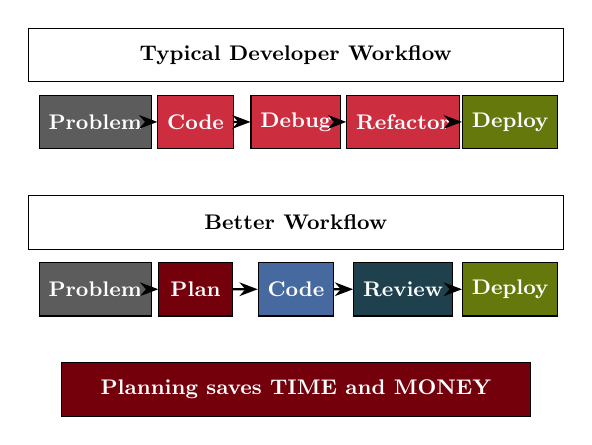
\begin{tikzpicture}[node distance=0.4cm, scale=0.85, transform shape]
                % Typical workflow
                \node[lightbox, minimum width=8cm, minimum height=0.8cm] (typical) at (0,2) {\textbf{Typical Developer Workflow}};
                \node[box=UofSC70Black, minimum width=1.3cm] (p1) at (-3,1) {Problem};
                \node[box=UofSCRose, minimum width=1.1cm] (c1) at (-1.5,1) {Code};
                \node[box=UofSCRose, minimum width=1.1cm] (d1) at (0,1) {Debug};
                \node[box=UofSCRose, minimum width=1.3cm] (r1) at (1.6,1) {Refactor};
                \node[box=UofSCHorseshoe, minimum width=1.1cm] (dep1) at (3.2,1) {Deploy};

                \draw[arrow] (p1) -- (c1);
                \draw[arrow] (c1) -- (d1);
                \draw[arrow] (d1) -- (r1);
                \draw[arrow] (r1) -- (dep1);

                % Better workflow
                \node[lightbox, minimum width=8cm, minimum height=0.8cm] (better) at (0,-0.5) {\textbf{Better Workflow}};
                \node[box=UofSC70Black, minimum width=1.3cm] (p2) at (-3,-1.5) {Problem};
                \node[box=UofSCGarnet, minimum width=1.1cm] (plan) at (-1.5,-1.5) {Plan};
                \node[box=UofSCAtlantic, minimum width=1.1cm] (c2) at (0,-1.5) {Code};
                \node[box=UofSCCongaree, minimum width=1.1cm] (rev) at (1.6,-1.5) {Review};
                \node[box=UofSCHorseshoe, minimum width=1.1cm] (dep2) at (3.2,-1.5) {Deploy};

                \draw[arrow] (p2) -- (plan);
                \draw[arrow] (plan) -- (c2);
                \draw[arrow] (c2) -- (rev);
                \draw[arrow] (rev) -- (dep2);

                % Result box
                \node[box=UofSCGarnet, minimum width=7cm, minimum height=0.8cm, text width=6.5cm] at (0,-3) {Planning saves TIME and MONEY};
            \end{tikzpicture}
            \end{center}
        \end{column}
        \begin{column}{0.42\textwidth}
            \begin{block}{Key Questions}
                \begin{itemize}
                    \item What are real costs of skipping planning?
                    \item How does planning improve code quality?
                    \item How do agentic tools amplify benefits?
                \end{itemize}
            \end{block}
            \vspace{0.3cm}
            \begin{alertblock}{Discussion}
                Think about the last time you started coding without a plan. What went wrong?
            \end{alertblock}
        \end{column}
    \end{columns}

    \note{Planning isn't about slowing down---it's about directing effort productively. With agentic tools, planning becomes even more critical because agents can generate large amounts of code rapidly.}
\end{frame}

\begin{frame}{The Cost of Skipping Planning}
    \begin{columns}[T]
        \begin{column}{0.48\textwidth}
            \begin{block}{Wasted Effort}
                \begin{itemize}
                    \item Code written but never used ($\sim$30\%)
                    \item Rework and refactoring cycles
                    \item Dead ends and false starts
                \end{itemize}
            \end{block}
            \begin{block}{Architectural Problems}
                \begin{itemize}
                    \item Structural incompatibilities
                    \item Poor scalability decisions
                    \item Tight coupling and dependencies
                \end{itemize}
            \end{block}
        \end{column}
        \begin{column}{0.48\textwidth}
            \begin{block}{Quality Issues}
                \begin{itemize}
                    \item More bugs (80\% logic errors)
                    \item Harder to test
                    \item Difficult to maintain
                \end{itemize}
            \end{block}
            \begin{block}{Team Communication}
                \begin{itemize}
                    \item Unclear requirements
                    \item Wrong assumptions
                    \item Conflicting implementations
                \end{itemize}
            \end{block}
        \end{column}
    \end{columns}
    \vspace{0.3cm}
    \begin{alertblock}{With Agentic Tools}
        Without planning, agents amplify waste---generating pages of incorrect code in seconds.
    \end{alertblock}

    \note{Studies show 30-40\% of code in unplanned projects is discarded. Key costs: wasted code, architecture issues, 3-4x higher defect density, and team coordination problems.}
\end{frame}

\begin{frame}{How Planning Improves Results}
    \begin{center}
    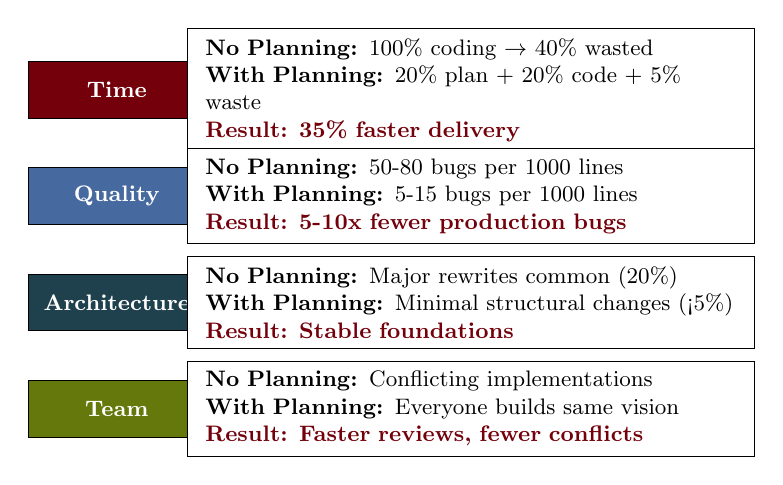
\begin{tikzpicture}[scale=0.9, transform shape]
        % Time efficiency
        \node[box=UofSCGarnet, minimum width=2.5cm] (t1) at (0,2.5) {Time};
        \node[lightbox, minimum width=8cm, text width=7.5cm, align=left] at (5,2.5) {
            \textbf{No Planning:} 100\% coding $\rightarrow$ 40\% wasted\\
            \textbf{With Planning:} 20\% plan + 20\% code + 5\% waste\\
            \textcolor{UofSCGarnet}{\textbf{Result: 35\% faster delivery}}
        };

        % Code quality
        \node[box=UofSCAtlantic, minimum width=2.5cm] (q1) at (0,1) {Quality};
        \node[lightbox, minimum width=8cm, text width=7.5cm, align=left] at (5,1) {
            \textbf{No Planning:} 50-80 bugs per 1000 lines\\
            \textbf{With Planning:} 5-15 bugs per 1000 lines\\
            \textcolor{UofSCGarnet}{\textbf{Result: 5-10x fewer production bugs}}
        };

        % Architecture
        \node[box=UofSCCongaree, minimum width=2.5cm] (a1) at (0,-0.5) {Architecture};
        \node[lightbox, minimum width=8cm, text width=7.5cm, align=left] at (5,-0.5) {
            \textbf{No Planning:} Major rewrites common (20\%)\\
            \textbf{With Planning:} Minimal structural changes (<5\%)\\
            \textcolor{UofSCGarnet}{\textbf{Result: Stable foundations}}
        };

        % Team
        \node[box=UofSCHorseshoe, minimum width=2.5cm] (team) at (0,-2) {Team};
        \node[lightbox, minimum width=8cm, text width=7.5cm, align=left] at (5,-2) {
            \textbf{No Planning:} Conflicting implementations\\
            \textbf{With Planning:} Everyone builds same vision\\
            \textcolor{UofSCGarnet}{\textbf{Result: Faster reviews, fewer conflicts}}
        };
    \end{tikzpicture}
    \end{center}

    \note{McConnell's ``Code Complete'' shows planning reduces defect density by 5-10x. IEEE studies show planned projects finish 25-30\% faster.}
\end{frame}

\begin{frame}{Research Evidence for Planning Benefits}
    \begin{columns}[T]
        \begin{column}{0.48\textwidth}
            \begin{exampleblock}{NASA Software Quality Data}
                \begin{itemize}
                    \item With design reviews: 0.5 defects/KLOC
                    \item Without design phase: 4.5 defects/KLOC
                    \item \textbf{Result: 9x more defects without planning}
                \end{itemize}
            \end{exampleblock}
            \vspace{0.2cm}
            \begin{exampleblock}{Microsoft Code Review (2016)}
                \begin{itemize}
                    \item With design discussions: 12\% revision rate
                    \item Without discussions: 43\% revision rate
                    \item \textbf{Result: 3.6x more revisions}
                \end{itemize}
            \end{exampleblock}
        \end{column}
        \begin{column}{0.48\textwidth}
            \begin{exampleblock}{Google Large-Scale Changes}
                \begin{itemize}
                    \item With 1-2 week planning: 95\% first-submit acceptance
                    \item Without planning: 62\% acceptance
                    \item \textbf{Result: 3x higher acceptance rate}
                \end{itemize}
            \end{exampleblock}
            \vspace{0.2cm}
            \begin{exampleblock}{Stack Overflow Survey 2024}
                \begin{itemize}
                    \item Developers who plan: 23\% higher satisfaction
                    \item Features delivered 30\% faster
                    \item Less frustration and rework
                \end{itemize}
            \end{exampleblock}
        \end{column}
    \end{columns}

    \note{With agentic tools, these benefits are even more pronounced because agents can quickly implement poor designs, making planning essential.}
\end{frame}

\begin{frame}{Planning Anti-patterns}
    \begin{columns}[T]
        \begin{column}{0.48\textwidth}
            \begin{alertblock}{1. Over-Planning}
                60\% planning, 40\% implementation\\
                Creates outdated specs, kills flexibility
            \end{alertblock}
            \begin{alertblock}{2. Planning in Isolation}
                One person plans, rest code\\
                Misses practitioner input and feasibility
            \end{alertblock}
            \begin{alertblock}{3. Planning Without Research}
                Assume domain knowledge\\
                Miss existing solutions and constraints
            \end{alertblock}
        \end{column}
        \begin{column}{0.48\textwidth}
            \begin{alertblock}{4. Static Plans}
                Plan once, follow forever\\
                Cannot adapt to discoveries
            \end{alertblock}
            \begin{alertblock}{5. No Validation}
                Plan but never test feasibility\\
                Discover problems during implementation
            \end{alertblock}
            \vspace{0.3cm}
            \begin{block}{With Agentic Tools}
                These anti-patterns are amplified because agents execute plans rapidly---bad plans get implemented at scale.
            \end{block}
        \end{column}
    \end{columns}

    \note{It's not about planning more---it's about planning well. With agentic tools, bad plans become bad code very quickly.}
\end{frame}

\begin{frame}{The Planning-Building Mindset}
    \begin{center}
    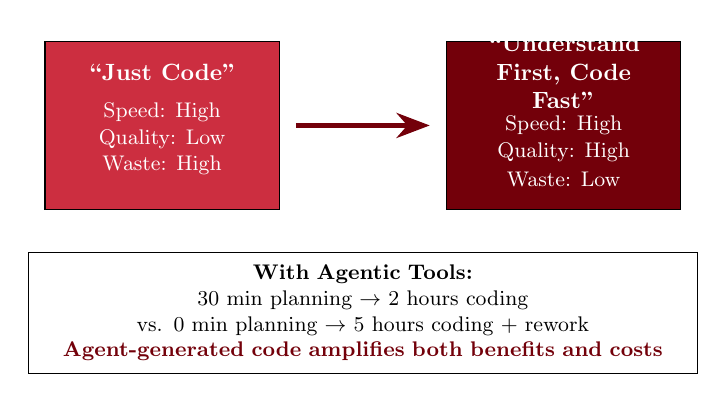
\begin{tikzpicture}[scale=0.85, transform shape]
        % Old mindset
        \node[box=UofSCRose, minimum width=3.5cm, minimum height=2.5cm] (old) at (-4,0) {};
        \node[text=UofSCWhite, font=\bfseries] at (-4,0.8) {``Just Code''};
        \node[text=UofSCWhite, font=\small] at (-4,0.2) {Speed: High};
        \node[text=UofSCWhite, font=\small] at (-4,-0.2) {Quality: Low};
        \node[text=UofSCWhite, font=\small] at (-4,-0.6) {Waste: High};

        % Arrow
        \draw[bigarrow, line width=2pt] (-2,0) -- (0,0);

        % New mindset
        \node[box=UofSCGarnet, minimum width=3.5cm, minimum height=2.5cm] (new) at (2,0) {};
        \node[text=UofSCWhite, font=\bfseries, text width=3cm, align=center] at (2,0.8) {``Understand First, Code Fast''};
        \node[text=UofSCWhite, font=\small] at (2,0) {Speed: High};
        \node[text=UofSCWhite, font=\small] at (2,-0.4) {Quality: High};
        \node[text=UofSCWhite, font=\small] at (2,-0.8) {Waste: Low};

        % Bottom box
        \node[lightbox, minimum width=10cm, minimum height=1.8cm, text width=9.5cm] at (-1,-2.8) {
            \textbf{With Agentic Tools:}\\
            30 min planning $\rightarrow$ 2 hours coding\\
            vs. 0 min planning $\rightarrow$ 5 hours coding + rework\\
            \textcolor{UofSCGarnet}{\textbf{Agent-generated code amplifies both benefits and costs}}
        };
    \end{tikzpicture}
    \end{center}

    \vspace{0.2cm}
    \begin{block}{Time Allocation Target}
        10-20\% planning $\bullet$ 70-80\% implementing $\bullet$ 5-10\% reviewing
    \end{block}

    \note{Planning is not the opposite of speed---it's the path to sustainable speed. Planning isn't a delay, it's an acceleration.}
\end{frame}

%==============================================================================
% SECTION 2: Research-Plan-Implement-Review Pattern
%==============================================================================
\section{The Research-Plan-Implement-Review Pattern}

\begin{frame}{The Research-Plan-Implement-Review Cycle}
    \begin{center}
    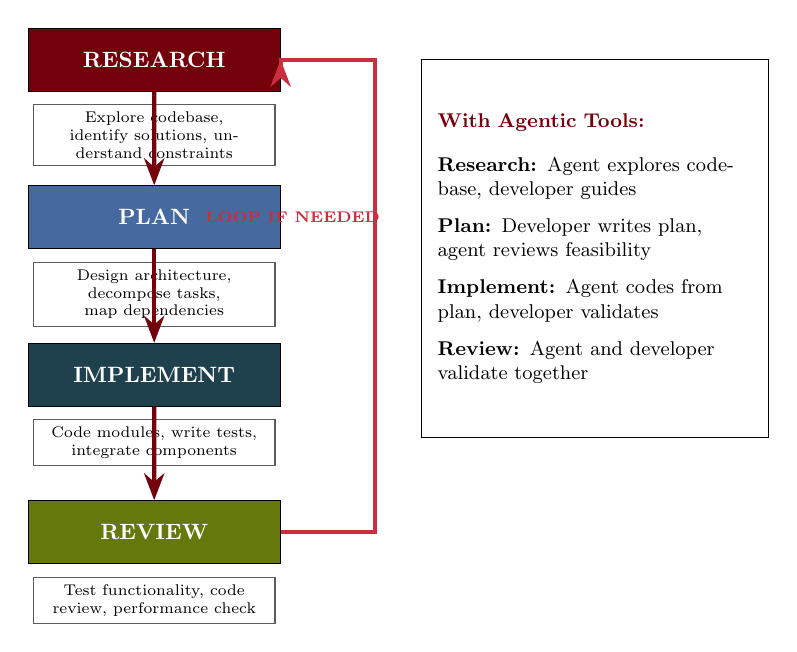
\begin{tikzpicture}[node distance=1.8cm, scale=0.8, transform shape]
        % Research phase
        \node[phase=UofSCGarnet, minimum width=4cm] (research) at (0,3) {RESEARCH};
        \node[subphase, below=0.2cm of research, minimum width=3.8cm, text width=3.6cm] (r1) {Explore codebase, identify solutions, understand constraints};

        % Plan phase
        \node[phase=UofSCAtlantic, minimum width=4cm] (plan) at (0,0.5) {PLAN};
        \node[subphase, below=0.2cm of plan, minimum width=3.8cm, text width=3.6cm] (p1) {Design architecture, decompose tasks, map dependencies};

        % Implement phase
        \node[phase=UofSCCongaree, minimum width=4cm] (impl) at (0,-2) {IMPLEMENT};
        \node[subphase, below=0.2cm of impl, minimum width=3.8cm, text width=3.6cm] (i1) {Code modules, write tests, integrate components};

        % Review phase
        \node[phase=UofSCHorseshoe, minimum width=4cm] (review) at (0,-4.5) {REVIEW};
        \node[subphase, below=0.2cm of review, minimum width=3.8cm, text width=3.6cm] (rev1) {Test functionality, code review, performance check};

        % Arrows
        \draw[bigarrow] (research) -- (plan);
        \draw[bigarrow] (plan) -- (impl);
        \draw[bigarrow] (impl) -- (review);

        % Loop back arrow
        \draw[bigarrow, UofSCRose] (review.east) -- ++(1.5,0) -- ++(0,7.5) -- ++(-1.5,0) -- (research.east);
        \node[text=UofSCRose, font=\scriptsize\bfseries] at (2.2,0.5) {LOOP IF NEEDED};

        % Right side - with agentic tools
        \node[lightbox, minimum width=5.5cm, minimum height=6cm, text width=5cm, align=left] at (7,0) {
            \textbf{\textcolor{UofSCGarnet}{With Agentic Tools:}}\\[0.3cm]
            \textbf{Research:} Agent explores codebase, developer guides\\[0.2cm]
            \textbf{Plan:} Developer writes plan, agent reviews feasibility\\[0.2cm]
            \textbf{Implement:} Agent codes from plan, developer validates\\[0.2cm]
            \textbf{Review:} Agent and developer validate together
        };
    \end{tikzpicture}
    \end{center}

    \note{This pattern is iterative---each phase informs the others. Unlike waterfall, you loop back when needed.}
\end{frame}

\begin{frame}{Research Phase: Understanding Your Problem}
    \begin{columns}[T]
        \begin{column}{0.48\textwidth}
            \begin{block}{1. Understand the Domain}
                \begin{itemize}
                    \item What problem are you solving?
                    \item Who is the user?
                    \item What are the constraints?
                    \item What's the success criteria?
                \end{itemize}
            \end{block}
            \begin{block}{2. Explore the Codebase}
                \begin{itemize}
                    \item How is related code structured?
                    \item What patterns and conventions?
                    \item What can you reuse?
                \end{itemize}
            \end{block}
        \end{column}
        \begin{column}{0.48\textwidth}
            \begin{block}{3. Identify Constraints}
                \begin{itemize}
                    \item Performance requirements
                    \item Scalability needs
                    \item Security considerations
                \end{itemize}
            \end{block}
            \begin{block}{Agent's Role in Research}
                \begin{itemize}
                    \item Search codebase for patterns
                    \item Find similar implementations
                    \item Identify relevant code sections
                    \item Verify your assumptions
                \end{itemize}
            \end{block}
        \end{column}
    \end{columns}
    \vspace{0.2cm}
    \begin{alertblock}{Red Flags During Research}
        Conflicting requirements not identified $\bullet$ Missing critical constraints $\bullet$ Overlooked existing solutions
    \end{alertblock}

    \note{With agentic tools, agents can help dramatically by searching codebases, finding patterns, and identifying similar implementations. However, the developer must guide this research.}
\end{frame}

\begin{frame}{Planning Phase: Designing Your Solution}
    \begin{center}
    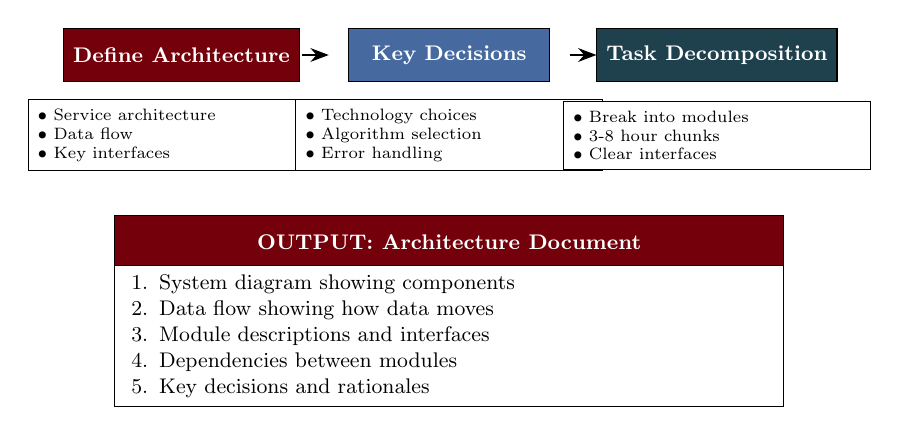
\begin{tikzpicture}[scale=0.85, transform shape]
        % Step boxes
        \node[box=UofSCGarnet, minimum width=3cm] (s1) at (-4,2.5) {Define Architecture};
        \node[lightbox, minimum width=4.5cm, text width=4.3cm, align=left, font=\scriptsize] at (-4,1.3) {
            $\bullet$ Service architecture\\
            $\bullet$ Data flow\\
            $\bullet$ Key interfaces
        };

        \node[box=UofSCAtlantic, minimum width=3cm] (s2) at (0,2.5) {Key Decisions};
        \node[lightbox, minimum width=4.5cm, text width=4.3cm, align=left, font=\scriptsize] at (0,1.3) {
            $\bullet$ Technology choices\\
            $\bullet$ Algorithm selection\\
            $\bullet$ Error handling
        };

        \node[box=UofSCCongaree, minimum width=3cm] (s3) at (4,2.5) {Task Decomposition};
        \node[lightbox, minimum width=4.5cm, text width=4.3cm, align=left, font=\scriptsize] at (4,1.3) {
            $\bullet$ Break into modules\\
            $\bullet$ 3-8 hour chunks\\
            $\bullet$ Clear interfaces
        };

        % Arrows between steps
        \draw[arrow, thick] (-2.2,2.5) -- (-1.8,2.5);
        \draw[arrow, thick] (1.8,2.5) -- (2.2,2.5);

        % Output section
        \node[box=UofSCGarnet, minimum width=10cm, minimum height=0.8cm] at (0,-0.3) {OUTPUT: Architecture Document};
        \node[lightbox, minimum width=10cm, minimum height=1.8cm, text width=9.5cm, align=left] at (0,-1.7) {
            1. System diagram showing components\\
            2. Data flow showing how data moves\\
            3. Module descriptions and interfaces\\
            4. Dependencies between modules\\
            5. Key decisions and rationales
        };
    \end{tikzpicture}
    \end{center}

    \note{Planning phase translates research findings into concrete design. This is where you decide what to build and how it fits together.}
\end{frame}

\begin{frame}{Detailed Task Decomposition}
    \begin{columns}[T]
        \begin{column}{0.55\textwidth}
            \begin{exampleblock}{Example: API Request Caching Layer ($\sim$40h)}
                \textbf{Phase 1: Setup (12h)}
                \begin{itemize}
                    \item Task 1.1: Design architecture (2h)
                    \item Task 1.2: Testing infrastructure (3h)
                    \item Task 1.3: Dependency setup (2h)
                    \item Task 1.4: Documentation (5h)
                \end{itemize}
                \textbf{Phase 2: Core Implementation (20h)}
                \begin{itemize}
                    \item Task 2.1: Cache interface (3h)
                    \item Task 2.2: Redis implementation (5h)
                    \item Task 2.3: Invalidation system (4h)
                    \item Task 2.4: Performance optimization (5h)
                    \item Task 2.5: Monitoring (3h)
                \end{itemize}
            \end{exampleblock}
        \end{column}
        \begin{column}{0.42\textwidth}
            \begin{block}{Key Principles}
                \begin{enumerate}
                    \item \textbf{Independence:} Minimal dependencies
                    \item \textbf{Size:} 3-8 hour chunks
                    \item \textbf{Interfaces:} Clear inputs/outputs
                    \item \textbf{Testability:} Can test independently
                \end{enumerate}
            \end{block}
            \vspace{0.2cm}
            \begin{alertblock}{Red Flags}
                \begin{itemize}
                    \item Tasks $>$12 hours (too big)
                    \item Tasks $<$1 hour (too granular)
                    \item Circular dependencies
                    \item Unclear ``done'' criteria
                \end{itemize}
            \end{alertblock}
        \end{column}
    \end{columns}

    \note{Good task decomposition allows agents to implement each task independently, making testing clearer and integration simpler.}
\end{frame}

\begin{frame}{Implementation Phase: Building from Plans}
    \begin{center}
    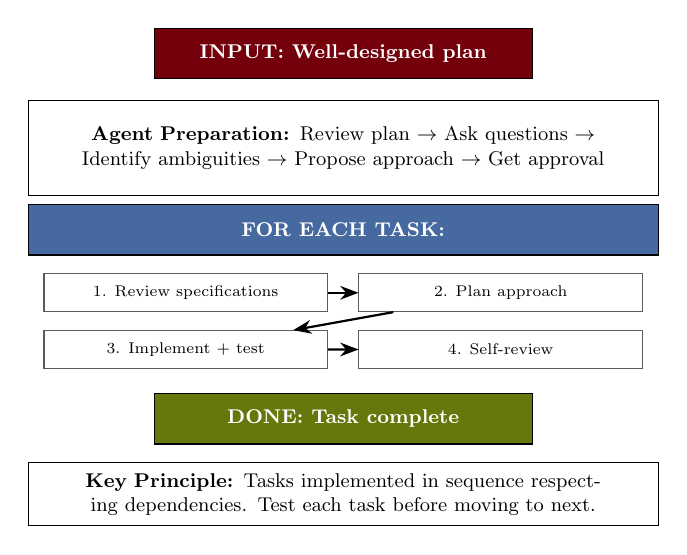
\begin{tikzpicture}[scale=0.8, transform shape]
        % Input
        \node[box=UofSCGarnet, minimum width=6cm] (input) at (0,3.5) {INPUT: Well-designed plan};

        % Preparation box
        \node[lightbox, minimum width=10cm, minimum height=1.5cm, text width=9.5cm] at (0,2) {
            \textbf{Agent Preparation:} Review plan $\rightarrow$ Ask questions $\rightarrow$ Identify ambiguities $\rightarrow$ Propose approach $\rightarrow$ Get approval
        };

        % For each task
        \node[box=UofSCAtlantic, minimum width=10cm] at (0,0.7) {FOR EACH TASK:};

        % Task steps
        \node[subphase, minimum width=4.5cm] (t1) at (-2.5,-0.3) {1. Review specifications};
        \node[subphase, minimum width=4.5cm] (t2) at (2.5,-0.3) {2. Plan approach};
        \node[subphase, minimum width=4.5cm] (t3) at (-2.5,-1.2) {3. Implement + test};
        \node[subphase, minimum width=4.5cm] (t4) at (2.5,-1.2) {4. Self-review};

        \draw[arrow] (t1) -- (t2);
        \draw[arrow] (t2) -- (t3);
        \draw[arrow] (t3) -- (t4);

        % Output
        \node[box=UofSCHorseshoe, minimum width=6cm] at (0,-2.3) {DONE: Task complete};

        % Key principle
        \node[lightbox, minimum width=10cm, minimum height=1cm, text width=9.5cm] at (0,-3.5) {
            \textbf{Key Principle:} Tasks implemented in sequence respecting dependencies. Test each task before moving to next.
        };
    \end{tikzpicture}
    \end{center}

    \note{Developer's role: Guide, Review, Validate, Adjust, Integrate. The agent is only as good as your specifications.}
\end{frame}

\begin{frame}{Review Phase: Validation and QA}
    \begin{columns}[T]
        \begin{column}{0.32\textwidth}
            \begin{block}{Testing Levels}
                \textbf{Level 1: Unit}\\
                Each module in isolation

                \textbf{Level 2: Integration}\\
                Modules tested together

                \textbf{Level 3: System}\\
                Full end-to-end testing

                \textbf{Level 4: Acceptance}\\
                Meets all requirements?
            \end{block}
        \end{column}
        \begin{column}{0.32\textwidth}
            \begin{block}{Review Checklist}
                \textcolor{UofSCGarnet}{$\square$} All requirements done\\
                \textcolor{UofSCGarnet}{$\square$} Edge cases handled\\
                \textcolor{UofSCGarnet}{$\square$} Test coverage $>$80\%\\
                \textcolor{UofSCGarnet}{$\square$} Code follows standards\\
                \textcolor{UofSCGarnet}{$\square$} API documented\\
                \textcolor{UofSCGarnet}{$\square$} Performance acceptable\\
                \textcolor{UofSCGarnet}{$\square$} No security issues
            \end{block}
        \end{column}
        \begin{column}{0.32\textwidth}
            \begin{alertblock}{Common Issues}
                \begin{itemize}
                    \item Missing edge cases
                    \item Poor error messages
                    \item Untested code paths
                    \item Performance issues
                    \item Security gaps
                \end{itemize}
            \end{alertblock}
        \end{column}
    \end{columns}
    \vspace{0.3cm}
    \begin{block}{Review Questions to Ask}
        ``What happens if this fails?'' $\bullet$ ``Can this be called with bad input?'' $\bullet$ ``What's worst-case performance?'' $\bullet$ ``Will the next developer understand this?''
    \end{block}

    \note{With agentic tools, review is especially important because agents generate code quickly and might not understand domain subtleties.}
\end{frame}

\begin{frame}{Complete Workflow Example: JWT Authentication}
    \begin{columns}[T]
        \begin{column}{0.48\textwidth}
            \begin{exampleblock}{Research Phase (2h)}
                \begin{itemize}
                    \item Found session-based auth exists
                    \item Identified backward compatibility need
                    \item Found existing error patterns
                    \item Clarified JWT requirements
                \end{itemize}
            \end{exampleblock}
            \begin{exampleblock}{Planning Phase (2h)}
                \begin{itemize}
                    \item Designed JWT service architecture
                    \item Key decision: Use PyJWT library
                    \item Task breakdown: 5 tasks, 16h total
                \end{itemize}
            \end{exampleblock}
        \end{column}
        \begin{column}{0.48\textwidth}
            \begin{exampleblock}{Implementation (16h)}
                \begin{itemize}
                    \item Task 1: JWT Service (4h) \checkmark
                    \item Task 2: Validation Middleware (3h) \checkmark
                    \item Task 3: Refresh Endpoint (2h) \checkmark
                    \item Task 4: Update Endpoints (3h) \checkmark
                    \item Task 5: Tests + Docs (4h) \checkmark
                \end{itemize}
            \end{exampleblock}
            \begin{exampleblock}{Review Phase (3h)}
                \begin{itemize}
                    \item 47 unit tests, 92\% coverage
                    \item 23 integration tests passing
                    \item All requirements verified
                \end{itemize}
            \end{exampleblock}
        \end{column}
    \end{columns}
    \vspace{0.2cm}
    \begin{block}{Result}
        \textbf{Total: 23 hours} (Estimated: 20h, Variance: +15\% --- within acceptable range)
    \end{block}

    \note{This example shows how research saved mistakes, clear planning made implementation straightforward, and comprehensive review verified everything works.}
\end{frame}

\begin{frame}{Common Pitfalls and How to Avoid Them}
    \begin{columns}[T]
        \begin{column}{0.48\textwidth}
            \begin{alertblock}{Pitfall: Skipping Research}
                \textbf{Symptom:} ``I know this codebase''\\
                \textbf{Risk:} Miss existing solutions\\
                \textbf{Fix:} Always spend 10-20\% on research
            \end{alertblock}
            \begin{alertblock}{Pitfall: Tasks Too Big}
                \textbf{Symptom:} ``Task 1: Implement entire system''\\
                \textbf{Risk:} Can't test incrementally\\
                \textbf{Fix:} Break into 3-8 hour chunks
            \end{alertblock}
            \begin{alertblock}{Pitfall: Missing Test Planning}
                \textbf{Symptom:} Tests thought of after\\
                \textbf{Risk:} Untestable code\\
                \textbf{Fix:} Plan tests with tasks
            \end{alertblock}
        \end{column}
        \begin{column}{0.48\textwidth}
            \begin{alertblock}{Pitfall: Planning Too Much}
                \textbf{Symptom:} 2-week plan for 1-week work\\
                \textbf{Risk:} Plan becomes outdated\\
                \textbf{Fix:} Plan just enough to start
            \end{alertblock}
            \begin{alertblock}{Pitfall: No Acceptance Criteria}
                \textbf{Symptom:} ``Task: implement caching''\\
                \textbf{Risk:} Unclear when done\\
                \textbf{Fix:} Define measurable criteria
            \end{alertblock}
            \begin{alertblock}{Pitfall: Agent Without Review}
                \textbf{Symptom:} Agent codes for 2h unreviewed\\
                \textbf{Risk:} Wrong direction\\
                \textbf{Fix:} Review frequently, feedback early
            \end{alertblock}
        \end{column}
    \end{columns}

    \note{With agentic tools, these pitfalls are even more dangerous because agents can rapidly amplify mistakes.}
\end{frame}

%==============================================================================
% SECTION 3: Plan Mode in Different Tools
%==============================================================================
\section{Plan Mode in Different Tools}

\begin{frame}{How Different Agentic Tools Support Planning}
    \begin{center}
    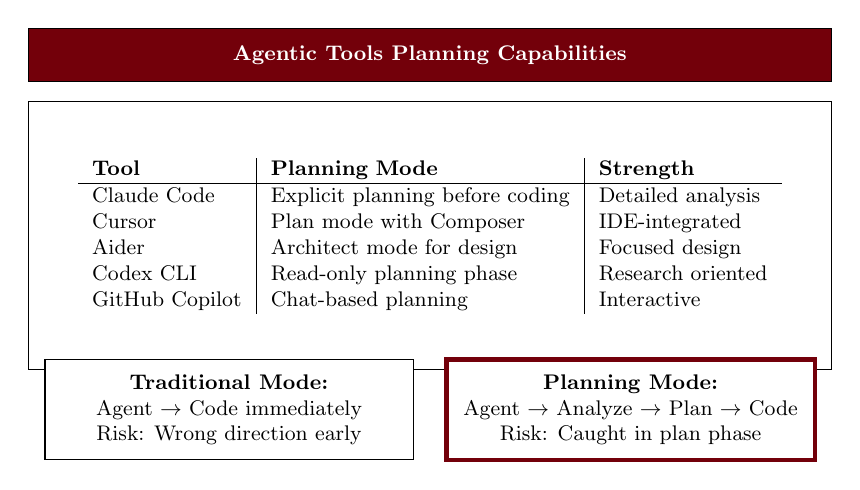
\begin{tikzpicture}[scale=0.85, transform shape]
        % Header
        \node[box=UofSCGarnet, minimum width=12cm] at (0,3) {Agentic Tools Planning Capabilities};

        % Table
        \node[lightbox, minimum width=12cm, minimum height=4cm, text width=11.5cm] at (0,0.3) {
            \begin{tabular}{l|l|l}
            \textbf{Tool} & \textbf{Planning Mode} & \textbf{Strength} \\
            \hline
            Claude Code & Explicit planning before coding & Detailed analysis \\
            Cursor & Plan mode with Composer & IDE-integrated \\
            Aider & Architect mode for design & Focused design \\
            Codex CLI & Read-only planning phase & Research oriented \\
            GitHub Copilot & Chat-based planning & Interactive \\
            \end{tabular}
        };

        % Bottom comparison
        \node[lightbox, minimum width=5.5cm, minimum height=1.5cm] at (-3,-2.3) {
            \textbf{Traditional Mode:}\\
            Agent $\rightarrow$ Code immediately\\
            Risk: Wrong direction early
        };
        \node[lightbox, minimum width=5.5cm, minimum height=1.5cm, draw=UofSCGarnet, line width=1.5pt] at (3,-2.3) {
            \textbf{Planning Mode:}\\
            Agent $\rightarrow$ Analyze $\rightarrow$ Plan $\rightarrow$ Code\\
            Risk: Caught in plan phase
        };
    \end{tikzpicture}
    \end{center}

    \note{Planning mode forces the agent to analyze before implementing, catching architectural issues before coding.}
\end{frame}

\begin{frame}{Claude Code: Explicit Planning Phase}
    \begin{columns}[T]
        \begin{column}{0.55\textwidth}
            \begin{center}
            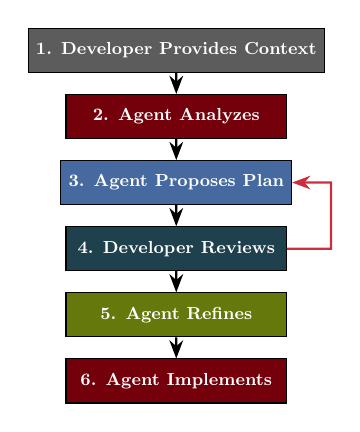
\begin{tikzpicture}[scale=0.7, transform shape, node distance=0.8cm]
                \node[box=UofSC70Black, minimum width=4cm] (c1) at (0,4) {1. Developer Provides Context};
                \node[box=UofSCGarnet, minimum width=4cm] (c2) at (0,2.8) {2. Agent Analyzes};
                \node[box=UofSCAtlantic, minimum width=4cm] (c3) at (0,1.6) {3. Agent Proposes Plan};
                \node[box=UofSCCongaree, minimum width=4cm] (c4) at (0,0.4) {4. Developer Reviews};
                \node[box=UofSCHorseshoe, minimum width=4cm] (c5) at (0,-0.8) {5. Agent Refines};
                \node[box=UofSCGarnet, minimum width=4cm] (c6) at (0,-2) {6. Agent Implements};

                \draw[arrow] (c1) -- (c2);
                \draw[arrow] (c2) -- (c3);
                \draw[arrow] (c3) -- (c4);
                \draw[arrow] (c4) -- (c5);
                \draw[arrow] (c5) -- (c6);

                % Feedback loop
                \draw[arrow, UofSCRose] (c4.east) -- ++(0.8,0) -- ++(0,1.2) -- (c3.east);
            \end{tikzpicture}
            \end{center}
        \end{column}
        \begin{column}{0.42\textwidth}
            \begin{block}{Plan Output Format}
                \begin{itemize}
                    \item High-level approach
                    \item Architecture overview
                    \item Task breakdown with estimates
                    \item Key decisions and rationales
                    \item Potential risks
                    \item Test strategy
                    \item Questions for clarification
                \end{itemize}
            \end{block}
            \begin{block}{Best For}
                Large features ($>$20h), architectural decisions, complex integrations
            \end{block}
        \end{column}
    \end{columns}

    \note{Claude Code's planning is designed for deep analysis and detailed planning. The agent explores your codebase and proposes comprehensive plans.}
\end{frame}

\begin{frame}{Getting Better Plans from Claude Code}
    \begin{columns}[T]
        \begin{column}{0.48\textwidth}
            \begin{block}{1. Provide Rich Context}
                \textbf{Good:} ``Add authentication''\\
                \textbf{Better:} ``FastAPI REST API needs JWT auth. Existing code uses [pattern]. Must support web and mobile.''
            \end{block}
            \begin{block}{2. Show Existing Patterns}
                \textbf{Good:} ``Follow conventions''\\
                \textbf{Better:} ``Here's our middleware [code], error pattern [code], testing approach [code]''
            \end{block}
            \begin{block}{3. Specify Constraints}
                \textbf{Good:} ``Must be performant''\\
                \textbf{Better:} ``Response $<$50ms, 20 DB connections max, backward compatible''
            \end{block}
        \end{column}
        \begin{column}{0.48\textwidth}
            \begin{block}{4. Define Success Criteria}
                \textbf{Good:} ``Make it work''\\
                \textbf{Better:} ``All 87 tests pass, $>$80\% coverage, mobile clients authenticate''
            \end{block}
            \begin{block}{5. Request Specific Sections}
                Ask for: Architecture diagram, task breakdown, key decisions, risks, test strategy, dependency graph, clarifying questions
            \end{block}
            \vspace{0.2cm}
            \begin{alertblock}{Iterate!}
                ``This approach is too complex''\\
                ``What if we used approach B?''\\
                ``How do we mitigate this risk?''
            \end{alertblock}
        \end{column}
    \end{columns}

    \note{The better your prompting and feedback, the better the plans. This is an investment that pays huge dividends in implementation quality.}
\end{frame}

\begin{frame}{Cursor: IDE-Integrated Planning}
    \begin{columns}[T]
        \begin{column}{0.48\textwidth}
            \begin{block}{Cursor Composer Workflow}
                \begin{enumerate}
                    \item Open Composer mode
                    \item Select files for context
                    \item Describe requirements
                    \item Review proposed diffs
                    \item Iterate or apply changes
                \end{enumerate}
            \end{block}
            \begin{exampleblock}{Strengths}
                \begin{itemize}
                    \item Visual context in IDE
                    \item File-aware planning
                    \item Interactive diffs
                    \item Immediate testing
                    \item Natural integration
                \end{itemize}
            \end{exampleblock}
        \end{column}
        \begin{column}{0.48\textwidth}
            \begin{alertblock}{Limitations}
                \begin{itemize}
                    \item Less detailed analysis
                    \item Better for local changes
                    \item Implicit planning
                    \item No task breakdown
                    \item Context window limits
                \end{itemize}
            \end{alertblock}
            \begin{block}{Best For}
                \begin{itemize}
                    \item Adding functions/methods
                    \item Refactoring existing code
                    \item Adding validation/utilities
                    \item Quick iterations
                \end{itemize}
            \end{block}
        \end{column}
    \end{columns}
    \vspace{0.2cm}
    \begin{block}{Cursor vs Claude Code}
        \textbf{Cursor:} Incremental changes, quick prototyping, local scope\\
        \textbf{Claude Code:} Large features, architecture, complex integrations
    \end{block}

    \note{Cursor's planning is more implicit and IDE-integrated. It's better for iterative changes within the IDE.}
\end{frame}

\begin{frame}{Aider: Terminal-Based Architecture Planning}
    \begin{columns}[T]
        \begin{column}{0.48\textwidth}
            \begin{block}{Aider Architect Workflow}
                \begin{enumerate}
                    \item \texttt{aider --architect}
                    \item Describe the feature
                    \item Architect analyzes codebase
                    \item Proposes solution
                    \item You review and decide
                    \item Aider implements
                \end{enumerate}
            \end{block}
            \begin{exampleblock}{Features}
                \begin{itemize}
                    \item Planning-first focus
                    \item Terminal integration
                    \item Version control aware
                    \item Conversational iteration
                    \item Makes atomic commits
                \end{itemize}
            \end{exampleblock}
        \end{column}
        \begin{column}{0.48\textwidth}
            \begin{block}{Example Session}
                \texttt{You:} ``Add rate limiting to API''\\[0.2cm]
                \texttt{Architect:} ``Analysis complete. Plan:
                \begin{itemize}
                    \item Create middleware
                    \item Use Redis for counts
                    \item Track per user/endpoint
                    \item Config-driven limits
                \end{itemize}
                Should I implement?''\\[0.2cm]
                \texttt{You:} ``What about anonymous users?''\\[0.2cm]
                \texttt{Architect:} ``Options: A) Deny B) Generous limit C) Rate by IP''
            \end{block}
        \end{column}
    \end{columns}
    \vspace{0.2cm}
    \begin{block}{Best For}
        Terminal-native developers $\bullet$ Feature planning $\bullet$ Architecture iteration $\bullet$ Git workflows
    \end{block}

    \note{Aider's architect mode is designed specifically for planning. It separates planning from implementation clearly.}
\end{frame}

\begin{frame}{Codex CLI: Research-Focused Planning}
    \begin{columns}[T]
        \begin{column}{0.48\textwidth}
            \begin{block}{Read-Only Mode Features}
                \textbf{Can Do:}
                \begin{itemize}
                    \item Search codebase
                    \item Analyze code patterns
                    \item Find similar implementations
                    \item Understand existing approaches
                    \item Document findings
                \end{itemize}
                \textbf{Cannot Do:}
                \begin{itemize}
                    \item Write or modify code
                    \item Commit changes
                    \item Run tests
                \end{itemize}
            \end{block}
        \end{column}
        \begin{column}{0.48\textwidth}
            \begin{exampleblock}{Research Prompts}
                ``Find all database queries for users''\\
                ``Show me caching implementations''\\
                ``What error handling patterns exist?''\\
                ``How is validation done?''\\
                ``What are performance requirements?''
            \end{exampleblock}
            \begin{block}{Workflow Position}
                \textbf{Step 1:} Codex research (read-only)\\
                \textbf{Step 2:} Claude Code planning\\
                \textbf{Step 3:} Aider/Cursor implementation
            \end{block}
        \end{column}
    \end{columns}
    \vspace{0.2cm}
    \begin{block}{Perfect For}
        Research phase $\bullet$ Exploring unfamiliar codebases $\bullet$ Finding patterns $\bullet$ Gathering requirements safely
    \end{block}

    \note{Codex's read-only mode is perfect for research---you get deep analysis without risk of accidentally modifying code.}
\end{frame}

\begin{frame}{Which Tool for Which Planning Task?}
    \begin{center}
    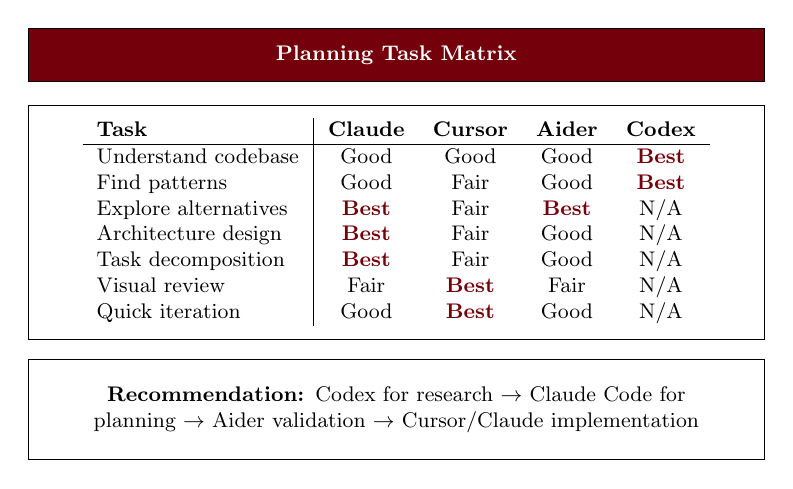
\begin{tikzpicture}[scale=0.85, transform shape]
        % Matrix header
        \node[box=UofSCGarnet, minimum width=11cm] at (0,3) {Planning Task Matrix};

        % Matrix content
        \node[lightbox, minimum width=11cm, minimum height=3.5cm, text width=10.5cm, font=\small] at (0,0.5) {
            \begin{tabular}{l|cccc}
            \textbf{Task} & \textbf{Claude} & \textbf{Cursor} & \textbf{Aider} & \textbf{Codex} \\
            \hline
            Understand codebase & Good & Good & Good & \textcolor{UofSCGarnet}{\textbf{Best}} \\
            Find patterns & Good & Fair & Good & \textcolor{UofSCGarnet}{\textbf{Best}} \\
            Explore alternatives & \textcolor{UofSCGarnet}{\textbf{Best}} & Fair & \textcolor{UofSCGarnet}{\textbf{Best}} & N/A \\
            Architecture design & \textcolor{UofSCGarnet}{\textbf{Best}} & Fair & Good & N/A \\
            Task decomposition & \textcolor{UofSCGarnet}{\textbf{Best}} & Fair & Good & N/A \\
            Visual review & Fair & \textcolor{UofSCGarnet}{\textbf{Best}} & Fair & N/A \\
            Quick iteration & Good & \textcolor{UofSCGarnet}{\textbf{Best}} & Good & N/A \\
            \end{tabular}
        };

        % Recommendation
        \node[lightbox, minimum width=11cm, minimum height=1.5cm, text width=10.5cm] at (0,-2.3) {
            \textbf{Recommendation:} Codex for research $\rightarrow$ Claude Code for planning $\rightarrow$ Aider validation $\rightarrow$ Cursor/Claude implementation
        };
    \end{tikzpicture}
    \end{center}

    \note{Don't try to force one tool to do everything. Use the right tool for each phase.}
\end{frame}

%==============================================================================
% SECTION 4: Plan-Act-Reflect Framework
%==============================================================================
\section{Plan-Act-Reflect Framework}

\begin{frame}{The Plan-Act-Reflect Cycle}
    \begin{center}
    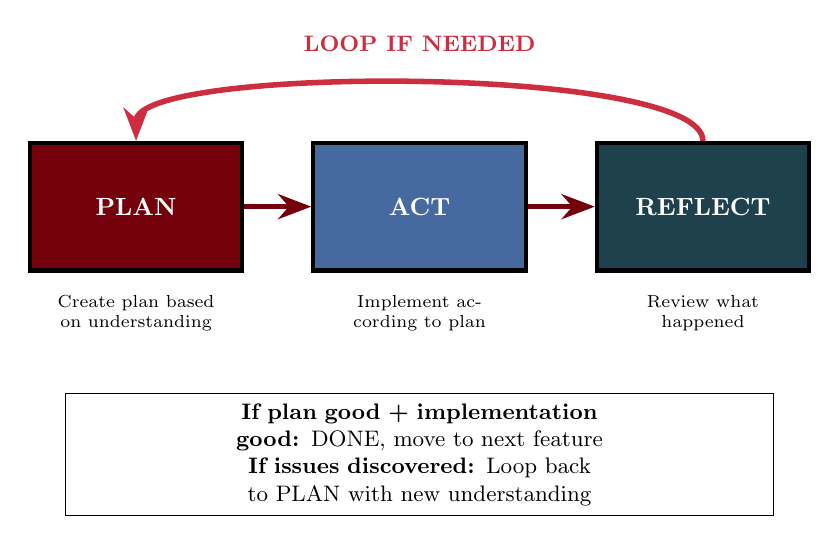
\begin{tikzpicture}[scale=0.9, transform shape]
        % Plan box
        \node[cyclebox=UofSCGarnet, minimum width=3cm, minimum height=1.8cm] (plan) at (-4,0) {PLAN};
        \node[font=\scriptsize, text width=2.8cm, align=center] at (-4,-1.5) {Create plan based on understanding};

        % Act box
        \node[cyclebox=UofSCAtlantic, minimum width=3cm, minimum height=1.8cm] (act) at (0,0) {ACT};
        \node[font=\scriptsize, text width=2.8cm, align=center] at (0,-1.5) {Implement according to plan};

        % Reflect box
        \node[cyclebox=UofSCCongaree, minimum width=3cm, minimum height=1.8cm] (reflect) at (4,0) {REFLECT};
        \node[font=\scriptsize, text width=2.8cm, align=center] at (4,-1.5) {Review what happened};

        % Arrows
        \draw[bigarrow, line width=2pt] (plan) -- (act);
        \draw[bigarrow, line width=2pt] (act) -- (reflect);
        \draw[bigarrow, line width=2pt, UofSCRose] (reflect.north) .. controls (4,2) and (-4,2) .. (plan.north);

        % Loop back label
        \node[text=UofSCRose, font=\small\bfseries] at (0,2.3) {LOOP IF NEEDED};

        % Decision box
        \node[lightbox, minimum width=10cm, minimum height=1.5cm, text width=9.5cm] at (0,-3.5) {
            \textbf{If plan good + implementation good:} DONE, move to next feature\\
            \textbf{If issues discovered:} Loop back to PLAN with new understanding
        };
    \end{tikzpicture}
    \end{center}

    \note{The Plan-Act-Reflect cycle is how continuous improvement happens. It's not just about building code---it's about getting better at building code.}
\end{frame}

\begin{frame}{Plan-Act-Reflect: Phase Details}
    \begin{columns}[T]
        \begin{column}{0.32\textwidth}
            \begin{block}{PLAN Phase}
                \textbf{Input:}\\
                Requirements, constraints, patterns

                \textbf{Activities:}\\
                Design architecture\\
                Break down tasks\\
                Create test strategy\\
                Identify risks

                \textbf{Output:}\\
                Architecture doc\\
                Task breakdown\\
                Risk analysis
            \end{block}
        \end{column}
        \begin{column}{0.32\textwidth}
            \begin{block}{ACT Phase}
                \textbf{Input:}\\
                Approved plan, task breakdown

                \textbf{Activities:}\\
                Implement each task\\
                Write tests\\
                Verify against spec\\
                Integrate components

                \textbf{Output:}\\
                Working code\\
                Test results\\
                Lessons learned
            \end{block}
        \end{column}
        \begin{column}{0.32\textwidth}
            \begin{block}{REFLECT Phase}
                \textbf{Input:}\\
                Completed implementation

                \textbf{Activities:}\\
                Compare to plan\\
                Analyze deviations\\
                Review quality\\
                Team feedback

                \textbf{Output:}\\
                Accept/reject decision\\
                Improvements identified
            \end{block}
        \end{column}
    \end{columns}
    \vspace{0.3cm}
    \begin{alertblock}{When to Loop Back}
        Major issues discovered $\bullet$ Requirements changed $\bullet$ Architecture problems found $\bullet$ Quality unacceptable
    \end{alertblock}

    \note{This cycle is used at multiple scales: per-task, per-feature, per-project, and across the organization.}
\end{frame}

\begin{frame}{Learning from Deviations}
    \begin{columns}[T]
        \begin{column}{0.48\textwidth}
            \begin{alertblock}{Deviation: Took Longer Than Planned}
                \textbf{Why?}
                \begin{itemize}
                    \item Estimate too optimistic
                    \item Unexpected complexity
                    \item Discovered new requirements
                \end{itemize}
                \textbf{Adjust:} Future plans more conservative
            \end{alertblock}
            \begin{alertblock}{Deviation: Code Quality Issues}
                \textbf{Why?}
                \begin{itemize}
                    \item Plan didn't address quality
                    \item Tests insufficient
                    \item Code review found issues
                \end{itemize}
                \textbf{Adjust:} Increase review/test in plan
            \end{alertblock}
        \end{column}
        \begin{column}{0.48\textwidth}
            \begin{alertblock}{Deviation: Architecture Issues}
                \textbf{Why?}
                \begin{itemize}
                    \item Original understanding wrong
                    \item Plan didn't match existing code
                    \item Missed integration point
                \end{itemize}
                \textbf{Adjust:} More planning time and depth
            \end{alertblock}
            \begin{block}{Questions to Ask in Reflection}
                \begin{itemize}
                    \item ``Are we on track?''
                    \item ``What have we learned?''
                    \item ``Do we need to adjust the plan?''
                    \item ``Are there emerging risks?''
                    \item ``Should we proceed or revise?''
                \end{itemize}
            \end{block}
        \end{column}
    \end{columns}

    \note{The reflection is where real learning happens. If you skip reflection, you repeat the same mistakes.}
\end{frame}

%==============================================================================
% SECTION 5: Static vs Dynamic Decomposition
%==============================================================================
\section{Static vs Dynamic Decomposition}

\begin{frame}{Static vs Dynamic Task Decomposition}
    \begin{center}
    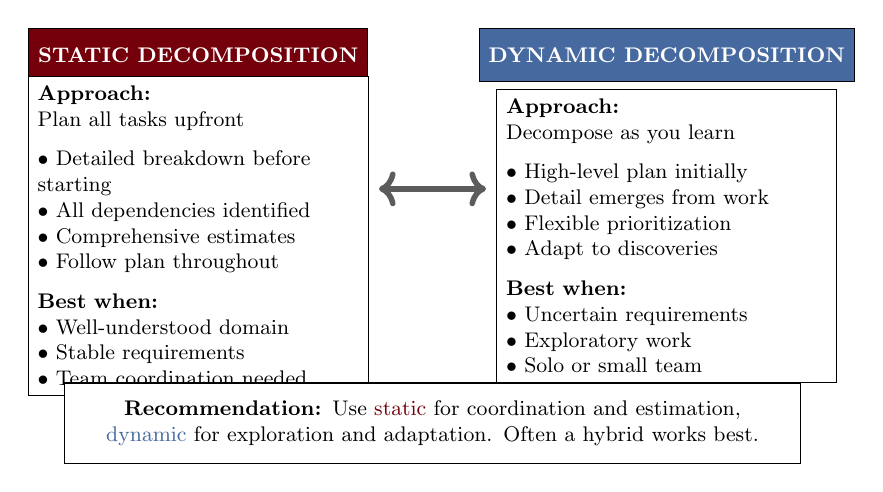
\begin{tikzpicture}[scale=0.85, transform shape]
        % Static side
        \node[box=UofSCGarnet, minimum width=5cm] at (-3.5,3) {STATIC DECOMPOSITION};
        \node[lightbox, minimum width=5cm, minimum height=4cm, text width=4.8cm, align=left] at (-3.5,0.3) {
            \textbf{Approach:}\\
            Plan all tasks upfront\\[0.2cm]
            $\bullet$ Detailed breakdown before starting\\
            $\bullet$ All dependencies identified\\
            $\bullet$ Comprehensive estimates\\
            $\bullet$ Follow plan throughout\\[0.2cm]
            \textbf{Best when:}\\
            $\bullet$ Well-understood domain\\
            $\bullet$ Stable requirements\\
            $\bullet$ Team coordination needed
        };

        % Dynamic side
        \node[box=UofSCAtlantic, minimum width=5cm] at (3.5,3) {DYNAMIC DECOMPOSITION};
        \node[lightbox, minimum width=5cm, minimum height=4cm, text width=4.8cm, align=left] at (3.5,0.3) {
            \textbf{Approach:}\\
            Decompose as you learn\\[0.2cm]
            $\bullet$ High-level plan initially\\
            $\bullet$ Detail emerges from work\\
            $\bullet$ Flexible prioritization\\
            $\bullet$ Adapt to discoveries\\[0.2cm]
            \textbf{Best when:}\\
            $\bullet$ Uncertain requirements\\
            $\bullet$ Exploratory work\\
            $\bullet$ Solo or small team
        };

        % Comparison arrow
        \draw[<->, line width=2pt, UofSC70Black] (-0.8,1) -- (0.8,1);

        % Bottom recommendation
        \node[lightbox, minimum width=11cm, minimum height=1.2cm, text width=10.5cm] at (0,-2.5) {
            \textbf{Recommendation:} Use \textcolor{UofSCGarnet}{static} for coordination and estimation, \textcolor{UofSCAtlantic}{dynamic} for exploration and adaptation. Often a hybrid works best.
        };
    \end{tikzpicture}
    \end{center}

    \note{Neither approach is universally better. Choose based on domain familiarity, requirement stability, and team size.}
\end{frame}

\begin{frame}{Comparing Decomposition Approaches}
    \begin{center}
    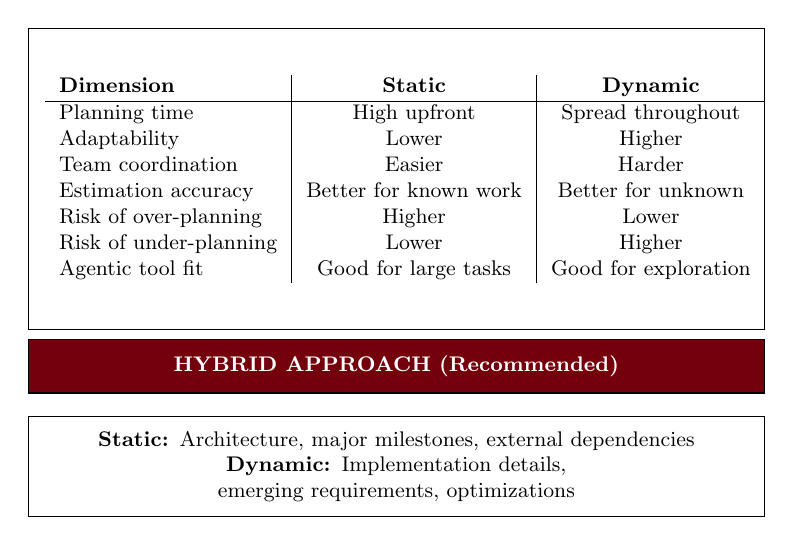
\begin{tikzpicture}[scale=0.85, transform shape]
        % Comparison table
        \node[lightbox, minimum width=11cm, minimum height=4.5cm, text width=10.5cm] at (0,0.5) {
            \begin{tabular}{l|c|c}
            \textbf{Dimension} & \textbf{Static} & \textbf{Dynamic} \\
            \hline
            Planning time & High upfront & Spread throughout \\
            Adaptability & Lower & Higher \\
            Team coordination & Easier & Harder \\
            Estimation accuracy & Better for known work & Better for unknown \\
            Risk of over-planning & Higher & Lower \\
            Risk of under-planning & Lower & Higher \\
            Agentic tool fit & Good for large tasks & Good for exploration \\
            \end{tabular}
        };

        % Hybrid approach
        \node[box=UofSCGarnet, minimum width=11cm] at (0,-2.3) {HYBRID APPROACH (Recommended)};
        \node[lightbox, minimum width=11cm, minimum height=1.5cm, text width=10.5cm] at (0,-3.8) {
            \textbf{Static:} Architecture, major milestones, external dependencies\\
            \textbf{Dynamic:} Implementation details, emerging requirements, optimizations
        };
    \end{tikzpicture}
    \end{center}

    \note{With agentic tools, static decomposition works well because agents can implement planned tasks quickly. But keep flexibility for discoveries.}
\end{frame}

%==============================================================================
% SECTION 6: Summary and Key Takeaways
%==============================================================================
\section{Summary}

\begin{frame}{Pattern Summary: Key Takeaways}
    \begin{columns}[T]
        \begin{column}{0.48\textwidth}
            \begin{block}{The Pattern}
                Research $\rightarrow$ Plan $\rightarrow$ Implement $\rightarrow$ Review $\rightarrow$ Loop
            \end{block}
            \begin{block}{Why It Works}
                \begin{itemize}
                    \item Research prevents missed context
                    \item Planning prevents wrong implementations
                    \item Implementation translates design to code
                    \item Review verifies everything works
                    \item Loop enables continuous improvement
                \end{itemize}
            \end{block}
            \begin{block}{Time Allocation}
                \begin{itemize}
                    \item Research: 10-15\%
                    \item Planning: 10-15\%
                    \item Implementation: 60-75\%
                    \item Review: 5-10\%
                \end{itemize}
            \end{block}
        \end{column}
        \begin{column}{0.48\textwidth}
            \begin{block}{With Agentic Tools}
                \begin{itemize}
                    \item Research: Agent helps explore faster
                    \item Planning: More detail = better agent output
                    \item Implementation: 40\% faster
                    \item Review: More important than ever
                \end{itemize}
            \end{block}
            \begin{alertblock}{Key Principle}
                \textbf{Good plans $\rightarrow$ good agent code}\\
                \textbf{Poor plans $\rightarrow$ poor agent code}\\[0.2cm]
                Planning skill becomes MORE important with agentic tools, not less.
            \end{alertblock}
        \end{column}
    \end{columns}

    \note{The cost of planning is small (10-15\%), but the benefit is large (40\%+ time savings). With agentic tools, this ratio improves even further.}
\end{frame}

\begin{frame}{When to Use This Pattern}
    \begin{columns}[T]
        \begin{column}{0.48\textwidth}
            \begin{block}{Always Use For}
                \begin{itemize}
                    \item New features ($>$1 day of work)
                    \item Architecture changes
                    \item Performance optimizations
                    \item Integration work
                    \item Complex bug fixes
                \end{itemize}
            \end{block}
            \begin{block}{Can Skip For}
                \begin{itemize}
                    \item Trivial fixes ($<$1 hour)
                    \item Simple bug fixes
                    \item Documentation updates
                    \item Routine refactoring
                \end{itemize}
            \end{block}
        \end{column}
        \begin{column}{0.48\textwidth}
            \begin{alertblock}{Don't Skip Because of...}
                \begin{itemize}
                    \item ``Just quick code''
                    \item ``I know this codebase''
                    \item ``Let's figure it out as we go''
                    \item ``Time pressure''
                \end{itemize}
                \vspace{0.2cm}
                \textbf{Time pressure makes planning MORE important, not less!}
            \end{alertblock}
            \vspace{0.3cm}
            \begin{block}{The Bottom Line}
                Planning is not the opposite of speed---it's the path to \textbf{sustainable speed}.
            \end{block}
        \end{column}
    \end{columns}

    \note{The goal is to instill a culture where developers spend 10-20\% of time planning, 70-80\% implementing, and 5-10\% reviewing.}
\end{frame}

\begin{frame}{Questions and Discussion}
    \begin{center}
    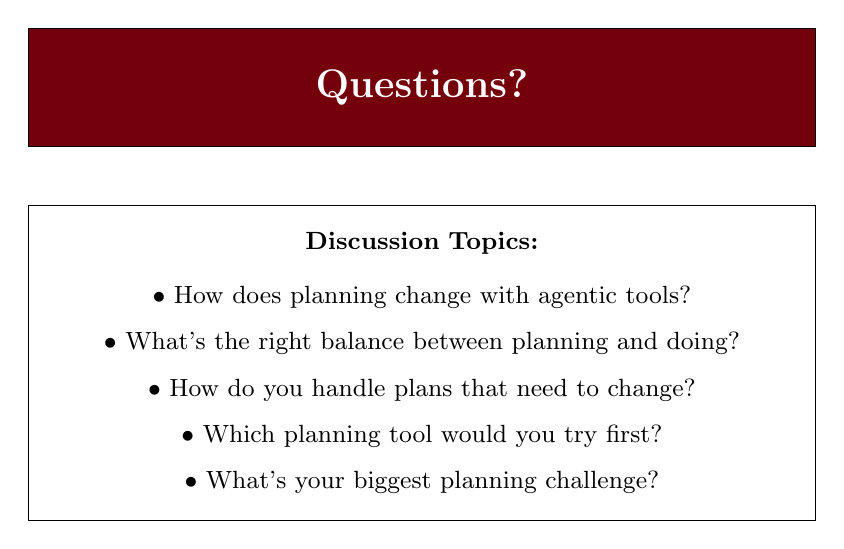
\begin{tikzpicture}
        \node[box=UofSCGarnet, minimum width=10cm, minimum height=1.5cm] at (0,2) {\Large Questions?};

        \node[lightbox, minimum width=10cm, minimum height=4cm, text width=9.5cm] at (0,-1.5) {
            \textbf{Discussion Topics:}\\[0.3cm]
            $\bullet$ How does planning change with agentic tools?\\[0.2cm]
            $\bullet$ What's the right balance between planning and doing?\\[0.2cm]
            $\bullet$ How do you handle plans that need to change?\\[0.2cm]
            $\bullet$ Which planning tool would you try first?\\[0.2cm]
            $\bullet$ What's your biggest planning challenge?
        };
    \end{tikzpicture}
    \end{center}

    \note{Encourage students to share their experiences with planning (or not planning) and how it affected their projects.}
\end{frame}

\end{document}
